\chapter{METODOLOGI}
\label{chap:metodologi}

% Ubah bagian-bagian berikut dengan isi dari desain dan implementasi

% Penelitian ini dilaksanakan sesuai dengan batasan-batasan masalah yang telah disebutkan
% pada bagian 1.3. Berikut ini adalah beberapa peralatan dan perangkat yang terlibat dalam
% penelitian ini.

\section{Metode yang Digunakan}
\label{sec:metodeyangdigunakan}

Tugas akhir ini merupakan penelitian di bidang visi komputer dengan tujuan untuk melakukan 
re-identifikasi mobil menggunakan kumpulan citra dari dataset VRIC. Alur blok diagram metodologi 
dapat dilihat pada gambar 3.1. Perancangan model menggunakan metode Swin Transformer dari 
\emph{Pytorch ReID layumi}.

\begin{figure}[ht]
  \centering
  % Nama dari file gambar yang diinputkan
  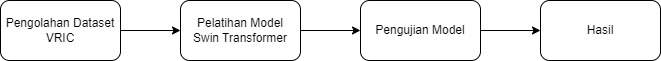
\includegraphics[scale=0.65]{gambar/metodologiFix.jpg}
  % Keterangan gambar yang diinputkan
  \caption{Diagram Blok Metodologi}
  % Label referensi dari gambar yang diinputkan
  \label{fig:diagramblokmetodologi}
\end{figure}

\begin{enumerate}[nolistsep]

  \item \textbf{Pengolahan Dataset VRIC}
  
  Pada tahapan ini, dilakukan proses pengolahan dataset yang didapat dengan 
  membagi dataset menjadi dua yaitu data training dan data test. Kedua data 
  ini nantinya akan digunakan untuk tujuan yang berbeda.

  \item \textbf{Pelatihan Model Swin Transformer}
  
  Pada tahapan ini, dilakukan training dan tuning pada model Swin Transformer 
  dengan mengubah parameternya. Parameter yang perlu disetel seperti 
  \emph{Loss Function}, \emph{Optimizer Function}, dan \emph{Epoch}.

  \item \textbf{Pengujian Model}
  
  Pada tahapan ini, model Swin Transformer yang telah melalui training dan 
  tuning akan diuji. Pengujian dilakukan menggunakan data test VRIC yang sebelumnya 
  telah dibagi.

  \item \textbf{Hasil}
  
  Jika hasil dari pengujian telah mencapai threshold dan model dapat melakukan \linebreak
  re-identifikasi dengan baik, maka seluruh hasil pengujian dicatat untuk dibandingkan 
  dengan penelitian yang sudah ada sebelumnya.

\end{enumerate}

\section{Bahan dan Peralatan yang Digunakan}
\label{sec:bahandanperalatanyangdigunakan}

\subsection{Dataset}

Dataset yang digunakan dalam penelitian ini adalah VRIC dataset. VRIC dataset memuat 
60 ribu citra mobil yang diambil dari kamera CCTV dari berbagai sudut pandang, sudut 
pencahayaan, dan kondisi lingkungan yang bermacam-macam. Setiap citra mobil dari VRIC 
dataset telah diberikan label sesuai dengan id vehicle dan id kamera yang mengambil 
citra tersebut.

%gambar 3.2 dataset

Gambar 3.2 merupakan beberapa contoh citra yang ada di VRIC dataset. Di dalam VRIC 
dataset, 60 ribu citra mobil telah dibagi ke tiga folder yang berbeda, yaitu folder 
\emph{train}, \emph{gallery}, dan \emph{query}. Folder \emph{train} berisikan 54 
ribu citra, sementara pada folder \emph{gallery} dan \emph{query} masing-masing 
berisikan 2 ribu citra. Terdapat pula list anotasi dari seluruh citra yang berisikan 
format nama file citra, label ID dari mobil, dan label kamera.

\subsection{Laptop}

Laptop digunakan untuk melakukan pemisahan (\emph{splitting}) dataset, training model, 
dan melakukan testing model yang telah selesai ditraining menggunakan VRIC dataset. 
Laptop perlu terhubung dengan internet untuk mengakses google Colaboratory, yang 
merupakan environment yang dibutuhkan untuk membuat model Swin Transformer. Spesifikasi 
laptop yang digunakan dapat dilihat pada tabel 3.1.

\begin{table}[ht]
  \begin{center}
  \caption{Spesifikasi Perangkat Laptop yang Digunakan}
  \label{tb:spesifikasilaptop}
  \begin{tabular}{|l|l|}
      \hline
      \textit{\textbf{Processor}}        & \begin{tabular}[c]{@{}l@{}}Intel Core i7-8750H \\ CPU @ 2.2 GHz\end{tabular} \\ \hline
      \textit{\textbf{Storage}}          & \begin{tabular}[c]{@{}l@{}}SSHD 1 TB Storage\\ SSD 128 GB Storage\end{tabular}         \\ \hline
      \textit{\textbf{RAM}}              & \begin{tabular}[c]{@{}l@{}}16 GB SODIMM DDR4 \\ 2666 MHz Dual Channel\end{tabular}    \\ \hline
      \textit{\textbf{Graphic Card}}     & \begin{tabular}[c]{@{}l@{}}NVIDIA GeForce GTX 1050 Ti \\ 4 GB GDDR5\end{tabular}      \\ \hline
      \textit{\textbf{Operating System}} & \begin{tabular}[c]{@{}l@{}}Windows 10 Home \\ Single Language 64-bit\end{tabular}     \\ \hline
  \end{tabular}
  \end{center}
\end{table}

\subsection{Google Colaboratory}

Google Colaboratory merupakan sebuah environment komputasi cloud dengan format \linebreak notebook 
yang disediakan oleh \emph{Google research} dengan fungsi untuk menjalankan kode python 
yang telah dituliskan. Google Colaboratory sangat membantu dalam pengerjaan \emph{data science}, 
\emph{deep learning}, dan \emph{machine learning} dikarenakan spesifikasi \emph{hardware} 
yang tinggi dari Google Colaboratory. Spesifikasi Google Colaboratory yang digunakan dapat 
dilihat pada tabel 3.2.

\begin{table}[ht]
  \begin{center}
  \caption{Spesifikasi Google Colaboratory}
  \label{tb:spesifikasigooglecolaboratory}
  \begin{tabular}{|l|l|}
      \hline
      \textit{\textbf{Processor}}        & \begin{tabular}[c]{@{}l@{}}Intel(R) Xeon(R) \\ CPU @ 2.2 GHz\end{tabular} \\ \hline
      \textit{\textbf{Graphic Card}}     & \begin{tabular}[c]{@{}l@{}}NVIDIA A100 SXM \\ 40 GB HBM2\end{tabular}      \\ \hline
  \end{tabular}
  \end{center}
\end{table}

\section{Urutan Pelaksanaan Penelitian}
\label{sec:urutanpelaksanaanpenelitian}

\subsection{Pemisahan Dataset}

VRIC dataset terbagi menjadi 3 bagian, yaitu data training, data query, dan data gallery. Ketiga 
bagian dataset tersebut telah dipisahkan dan disesuaikan secara langsung oleh developer dari VRIC 
dataset untuk kegunaan re-identifikasi mobil. Selain file berisi dataset, di dalam VRIC dataset 
juga terdapat file txt yang berisi list anotasi dari seluruh citra, dengan format nama file citra, 
label ID dari mobil, dan label kamera. Dengan menggunakan list anotasi tersebut, maka setiap dataset 
perlu dilakukan perubahan nama file sesuai dengan label ID dan label kameranya.

% Potongan kode rename
\lstinputlisting[
  language=Python,
  caption={Program Rename Dataset.},
  label={lst:renamedataset}
]{program/perubahan-nama-file.py}

Pada penelitian ini, diperlukan satu bagian lagi dalam percobaannya, yaitu data validasi. Data validasi 
berfungsi untuk melakukan validasi dan mengecek setiap epoch yang telah dilakukan pada training. Data 
validasi dibuat dengan mengambil sebagian data training untuk dipindahkan ke data validasi.

% Potongan kode splitting
\lstinputlisting[
  language=Python,
  caption={Program Pembagian Dataset.},
  label={lst:splittingdataset}
]{program/splitting-dataset.py}

\subsection{\emph{Training} dan \emph{Validation}}

\emph{Training} dilakukan setelah proses perubahan nama dan pemisahan dataset selesai dilakukan. Di dalam 
proses \emph{Training}, terdapat konfigurasi hyper-parameter yang harus ditentukan yaitu:

\begin{enumerate}[nolistsep]

  \item \textbf{Epoch}
  
  Epoch adalah hyper-parameter yang berfungsi untuk menentukan jumlah pengulangan proses \emph{learning} 
  yang harus dilakukan algoritma learning ke sebuah dataset training. Semakin banyaknya pengulangan yang 
  dilakukan maka model yang dihasilkan akan memiliki tingkat akurasi yang semakin tinggi, namun waktu 
  yang dibutuhkan dalam melakukan training juga akan semakin banyak.

  \item \textbf{\emph{Batch Size}}
  
  \emph{Batch size} adalah hyper-parameter yang berfungsi untuk mengontrol jumlah sampel \linebreak training 
  untuk dikerjakan sebelum parameter internal model diperbarui. Batch dapat dibayangkan seperti \emph{for-loop} 
  yang mengulang beberapa sampel dan kemudian membuat prediksi. Di akhir batch, prediksi dibandingkan 
  dengan variabel keluaran yang diharapkan dan kesalahan akan dihitung. Dari kesalahan ini, maka algoritma 
  pembaruan akan digunakan untuk memperbaiki model. 

  \item \textbf{\emph{Image Size}}
  
  \emph{Image size} merupakan dimensi ukuran citra yang diterapkan pada dataset. Ketika ukuran citra yang 
  diterapkan semakin kecil, maka waktu yang dibutuhkan untuk melakukan proses training akan semakin singkat. 

  \item \textbf{\emph{Learning Rate}}
  
  \emph{Learning rate} adalah hyper-parameter yang mengontrol besarnya perubahan suatu model dalam menanggapi 
  estimasi kesalahan setiap kali \emph{weight model} diperbarui. Dibutuhkan pemilihan nilai \emph{learning rate} 
  yang tepat karena ketika nilai yang digunakan terlalu kecil akan berdampak pada proses training yang terlalu 
  lama, sementara jika nilai yang digunakan terlalu besar mengakibatkan proses \emph{learning} kurang optimal.


  \item \textbf{\emph{Random Erasing Probability}}
  
  \emph{Random erasing probability} adalah hyper-parameter yang akan secara acak memilih sebagian wilayah dengan 
  bentuk persegi panjang kemudian menghapus pikselnya dengan nilai acak. \emph{Random erasing} melengkapi teknik 
  augmentasi data yang biasa digunakan seperti pemotongan dan pembalikan acak sehingga menghasilkan peningkatan yang 
  konsisten ketika digunakan di klasifikasi gambar, deteksi objek, dan re-identifikasi.

\end{enumerate}

\subsection{Model}

Penelitian ini akan menggunakan 2 jenis model, yaitu Swin Transformer V1 dan Swin Transformer V2 dengan ukuran model 
yang akan digunakan adalah model \emph{Base} (Swin-B). Kemudian akan dicoba pula menggunakan 2 format hyper-parameter yang 
berbeda. Sehingga akan dihasilkan 4 jenis model re-identifikasi mobil dengan pengaturan yang berbeda. Rincian hyper-parameter 
dapat dilihat pada tabel 3.3.

\begin{table}[ht]
  \begin{center}
  \caption{Rincian Model dan Hyper-Parameter dari Penelitian}
  \label{tb:rincianmodeldanhyperparameterdaripenelitian}
  \begin{tabular}{|l|l|l|}
      \hline
      \textit{ }        & \begin{tabular}[c]{@{}l@{}}\textbf{Swin Transformer V1}\end{tabular} & \begin{tabular}[c]{@{}l@{}}\textbf{Swin Transformer V2}\end{tabular}\\ \hline
      \textit{\textbf{Parameter 1}}  & \multicolumn{2}{|c|}{\parbox{6cm}{Batch Size=32; \\ Random Erasing Probability=0; \\ Learning Rate=0.05; \\ Warm Epoch=0}} \\ \hline
      \textit{\textbf{Parameter 2}}  & \multicolumn{2}{|c|}{\parbox{6cm}{Batch Size=16; \\ Random Erasing Probability=0.5; \\ Learning Rate=0.01; \\ Warm Epoch=5}} \\ \hline
      % \textit{\textbf{Parameter 1}}  & \begin{tabular}[c]{@{}l@{}}Batch Size=32 \\ Random Erasing Probability=0 \\ Learning Rate=0.05 \\ Warm Epoch=0\end{tabular} \\ \hline
      % \textit{\textbf{Parameter 2}}  & \begin{tabular}[c]{@{}l@{}}Batch Size=16 \\ Random Erasing Probability=0.5 \\ Learning Rate=0.01 \\ Warm Epoch=5\end{tabular} \\ \hline
  \end{tabular}
  \end{center}
\end{table}

\subsection{Pengujian Model}

Setiap model yang dibuat berdasarkan jenis model dan pengaturan hyper-parameternya akan diuji cobakan menggunakan data test 
dari dataset VRIC yang telah disiapkan. Hasil dari pengujian ini akan dicatat nilai akurasi ketepatan dari re-identifikasinya 
untuk setiap model dan akan dibandingkan hasil performanya. Dari pencatatan ini, nantinya dapat diketahui jenis model dan 
pengaturan hyper-parameter yang tepat untuk digunakan dalam re-identifikasi mobil.

% Alat diimplementasikan dengan \lipsum[1]

% % Contoh pembuatan potongan kode
% \begin{lstlisting}[
%   language=C++,
%   caption={Program halo dunia.},
%   label={lst:halodunia}
% ]
% #include <iostream>

% int main() {
%     std::cout << "Halo Dunia!";
%     return 0;
% }
% \end{lstlisting}

% \lipsum[2-3]

% % Contoh input potongan kode dari file
% \lstinputlisting[
%   language=Python,
%   caption={Program perhitungan bilangan prima.},
%   label={lst:bilanganprima}
% ]{program/bilangan-prima.py}

% \lipsum[4]
